%!TEX root = ../main.tex

\chapter{FFTbor2D}
\label{ch:ffttwo}

\lhead{FFTbor2D: 2D Coarse-Grained Energy Landscapes}

\section{Introduction}
\label{sec:ffttwo:intro}

In this chapter, we present the \ffttwo algorithm and accompanying software.
\ffttwo, like \fftbor described in \Chref{fftbor}, is an algorithm
which computes the paramerized partition function for an input RNA sequence
\seq. \ffttwo computes the two-dimensional coarse-grained energy landscape for \seq
given two compatible input secondary structures \strA and \strB, where position
$(x,y)$ on the discrete energy landscape corresponds to the Boltzmann
probability for those structures \str which have $\dBP{\str}{\strA}=x$ and
$\dBP{\str}{\strB}=y$ (where $d_{\text{BP}}$ is as defined in
equation \ref{eq:fftbor:dBP}). By again leveraging the \fft, \ffttwo runs in \On{5}
time and only uses \On{2} space---a significant improvement over previous
approaches. This permits the output energy landscape to be used in a
high-throughput fashion to analyze folding kinetics; a topic covered in detail
in \Chref{hermes}.

\subsection{Organization}
\label{subsec:ffttwo:org}

This chapter is organized in the following fashion. Because the history for
this work arises naturally from the history provided in
\Secref{sec:fftbor:bkgrnd}, we provide only a brief background
and immediately fall into
a technical discussion of the underlying algorithm. We first develop the
recursions for the Nussinov energy model for expository clarity, the
underlying implementation uses the more complicated and robust Turner energy
model. Recursions in place, we then move to show how these lead to
a single variable polynomial $P(x)$ whose coeffecients can be computed by
the \idft, and map to the 2D energy landscape. We describe two improvements over
the straight-forward use of the \fft to compute $P(x)$,
a parity condition and complex conjugates, which together reduce the
runtime by a factor of 4. Finally, we contrast this software against \rnatwofold,
and outline the performance characteristics of both softwares and highlight
the benefits and drawbacks of both. We elect to refrain from describing
applications of \ffttwo until \Chref{hermes}, where the software is
applied to quickly approximate \mfpt and \eqt for the folding of RNA molecules
between any two distinct, user provided structures \strAB.

\section{Background}
\label{sec:ffttwo:bkgrnd}

RNA folding pathways play an important role in biological processes.
For instance, in the {\em hok/sok}
(host-killing/suppression of killing) system \citep{gerdes.arg97},
the transition between two metastable RNA structures determines the
fate of a cell as follows.
The {\em hok} gene of {\em E. coli} and other bacteria
codes a small (52 amino acid) toxin causing irreversible damage to the cell
membrane. It has been shown that {\em hok}-mRNA is
constitutively expressed from a weak promoter, while
the rapidly degraded {\em sok}-RNA is constitutively expressed from
a strong promoter.  The {\em hok}-mRNA is initially
inactive, since a foldback sequesters the
Shine-Dalgarno sequence; however, slow exonucleolytic processing
digests the last $\approx 40$ nt of the $3'$ end of {\em hok}-mRNA,
transforming the molecule into its active form in which
the Shine-Dalgarno sequence is no longer sequestered.
If R1 plasmids of {\em E. coli} are present in
sufficient copy number, then a portion of the 64 nt
{\em sok}-RNA, which is complementary to {\em hok}-mRNA leader
region, binds to the active conformation of {\em hok}-mRNA, thus
causing degradation of the complex by RNase III \citep{gerdes.arg97}.
If plasmids are not present in sufficient copy number, then the
cell is killed by {\em hok} toxin, thus ensuring fitness of the daughter
cells.

In the case of spliced leader (SL) RNA from certain trypanosomes and nematodes,
a portion of the $5'$ exon is donated to
another mRNA by trans splicing.
Intermediate structures appear to be important in the process of splicing,
as shown by LeCuyer and Crothers \citep{lecuyercrothers}, who performed
stopped-flow rapid-mixing and temperature-jump measurements
of the kinetics for the structural transition between two low
energy structures of SL RNA from {\em Leptomonas collosoma}.
Conformational switches are thought not only to play a role in such
trans splicing, but as well in transcriptional and
translational regulation, protein synthesis, and mRNA splicing.

For these reasons, substantial experimental and computational work
has been done on folding pathways. In \citep{lorenz}, \rnatwofold---a dynamic
programming method that operates in
\On{7} time and \On{4} space---is presented, a generalization of \rnabor
\citep{freyhult.b07} that computes a 2D projection of the energy landscape,
discretized by \bpd to two input structures. Our work presented
here, called \ffttwo, produces a similar energy landscape in \On{5} time and
\On{2} space---efficient enough for the analysis of folding pathways of large
RNA sequences not tractable using \rnatwofold.

\section{Derivation of the \ffttwo algorithm}
\label{sec:ffttwo:math}

For expository clarity, we describe \ffttwo \citep{senter.jmb14}
and all recursions
in terms of the Nussinov energy model \citep{nussinovjacobson}
(same as in \Chref{fftbor}), where
the energy $E_0(i,j)$ of a base pair $(i,j)$ is defined to be $-1$, and the
energy $E(\str)$ of a secondary structure \str is $-1$ times the number $|\str|$
of base pairs in structure \str.  Nevertheless, the implementation of
\ffttwo involves the full Turner energy model \citep{xia:RNA}, where
free energy $E(\str)$ depends on negative, stabilizing energy contributions
from base stacking, and positive, destabilizing energy contributions due to
loss of entropy in loops.

\subsection{Definition of the partition function
\texorpdfstring{\bfZ{x,y}{1,n}}{}}
\label{subsec:ffttwo:recursions}

Given reference secondary structures \strAB of a
given RNA sequence $\seq=s_1,\dots,s_n$, our goal is to compute

\begin{align}
\label{eq:ffttwo:sumBoltzFactors}
\bfZ{x,y}{1,n}\;=\;
\sum_{\mathclap{\substack{
\str \text{ such that } \rule[-.5ex]{0pt}{0pt} \\
\dBP{\str}{\strA} = x,\,\dBP{\str}{\strB} = y}}}\enspace
\boltzF{\str}
\end{align}

for all $0 \leq x,y < n$, where $R$ is the universal gas constant, $T$
is absolute temperature, $E(\str)$ denotes the free energy of \str,
and \str ranges
over all secondary structures that are compatible with \seq. As mentioned,
we emphasize that for expository reasons alone, the Nussinov energy model is
used in the recursions in this chapter, although full recursions and
the implementation of \ffttwo, like \fftbor, involve the Turner energy model.

For any secondary structure \str of \seq, and any values
$1 \leq i \leq j \leq n$, the restriction $\str_{[i,j]}$ is defined to be the
collection of base pairs of \str, lying within interval $[i,j]$; i.e.
$\str_{[i,j]} = \{ (k, \ell) : i \leq k < \ell \leq j \}$.
In \citep{hofacker:RNAbor2D}, Lorenz et al. generalized
the dynamic programming recursions of our earlier work \citep{freyhult.b07},
to yield recursions
for the partition function $\bfZ{x,y}{i,j}$ in
\eqnref{ffttwo:sumBoltzFactors}. In the context of the Nussinov model,
$\bfZ{x,y}{i,j}$ is equal to

\begin{align}
\label{eq:ffttwo:bfZabij}
\begin{split}
& \bfZ{x-\alpha_0,y-\beta_0}{i,j-1}\enspace + \\
& \sum_{\substack{(s_k,s_j) \in \bpSet, \\ i \le k<j}}
\left(
\boltzNuss{k,j}\quad
\sum_{\mathclap{u+u'=x-\alpha(k)}}\hspace{3.75em}
\sum_{\mathclap{v+v'=y-\beta(k)}}\quad
\bfZ{u,v}{i,k-1} \cdot \bfZ{u',v'}{k+1,j-1}
\right)
\end{split}
\end{align}

where $\alpha_0 = 1$ if $j$ is base paired in $\strA_{[i,j]}$ and 0 otherwise,
$\beta_0 = 1$ if $j$ is base paired in $\strB_{[i,j]}$ and 0 otherwise,
$E_0(k,j)=-1$ if $k,j$ can base-pair
(see equation \ref{eq:fftbor:validBP}), and otherwise $E_0(k,j)=0$, and
$\alpha(k) =
\dBP{\strA_{[i,j]}}{\strA_{[i,k-1]} \cup \strA_{[k+1,j-1]} \cup \{ (k,j) \}}$,
and
$\beta(k) =
\dBP{\strB_{[i,j]}}{\strB_{[i,k-1]} \cup \strB_{[k+1,j-1]} \cup \{ (k,j) \}}$.

\subsection{Recursions to compute the polynomial
\texorpdfstring{\emZ{i,j}}{}}
\label{subsec:ffttwo:polynomial}

Given RNA sequence $\seq = s_1,\dots,s_n$
and two arbitrary, but fixed reference
structures \strAB, we define the {\em polynomial}

\begin{align}
\label{eq:ffttwo:zOfX}
\fullZx = \sum_{r=0}^{n-1} \sum_{s=0}^{n-1}\; z_{rn+s} x^{rn+s}
\end{align}

where (constant) coefficients

\begin{align}
z_{rn+s} = \bfZ{r,s}{1,n}\;=
\enspace\sum_{\mathclap{\substack{
\str \text{ such that } \rule[-.5ex]{0pt}{0pt} \\
\dBP{\str}{\strA} = r,\,\dBP{\str}{\strB} = s
}}}\enspace
\boltzF{\str}
\end{align}

where $E(\str)$ denotes the free energy of \str.
If we evaluate the polynomial \fullZx at $n^2$ distinct pairs of values
$a_0,\dots,a_{n^2-1}$ in

\begin{align}
\label{eq:ffttwo:solutionsForAlpha}
\emZof{}{a_0} = y_{0}, \dots, \emZof{}{a_{n^2-1}} = y_{n^2-1},
\end{align}

then Lagrange polynomial interpolation
(\eqnref{fftbor:lagrangeInterpolation})
guarantees that we can determine the coefficients $z_{rn+s}$ of \fullZx,
for $0 \leq r,s < n$. Due to technical difficulties concerning numerical
robustness observered while working on the \fftbor software
(\Chref{fftbor}), we will perform polynomial interpolation
by using Vandermonde matrices and the \fft (FFT).

The following theorem shows that a
recursion, analogous to \eqnref{ffttwo:bfZabij},
can be used to compute
the {\em polynomial} $\emZ{i,j}$ defined by

\begin{align}
\label{eq:ffttwo:emZij}
\emZ{i,j} &= \sum_{r=0}^{n-1} \sum_{s=0}^{n-1}\;
z_{rn+s}(i,j) \cdot x^{rn+s}\; =
\sum_{k=0}^{n^2-1} z_{k}(i,j) \cdot x^{k}
\end{align}

where

\begin{align}
z_{rn+s}(i,j) \;=\; \bfZ{r,s}{i,j}\;=
\enspace\sum_{\mathclap{\substack{
\str \text{ such that } \rule[-.5ex]{0pt}{0pt} \\
\dBP{\str}{\strA} = r,\,\dBP{\str}{\strB} = s
}}}\enspace
\boltzF{\str}.
\end{align}

Here, in the summation, \str runs over structures on $s_i,\dots,s_j$, which
are $r$-neighbors of the restriction $\strA_{[i,j]}$ of reference structure
\strA to interval $[i,j]$, and simultaneously
\str-neighbors of the restriction $\strB_{[i,j]}$ of reference structure
\strB to interval $[i,j]$.

\begin{theorem}
\label{thm:ffttwo:recursions}
Let $s_1,\dots,s_n$ be a given RNA sequence.
For any integers $1 \leq i < j \leq n$, let

\begin{align}
\emZ{i,j} = \sum_{r=0}^{n-1} \sum_{s=0}^{n-1}\; z_{rn+s} x^{rn+s}
\end{align}

where

\begin{align}
z_{rn+s}(i,j) = \bfZ{r,s}{i,j}.
\end{align}

Inductively we define $\emZ{i,j}$ to equal

\begin{align}
\label{eq:ffttwo:polyRecNussJac}
\begin{split}
&\emZof{i,j-1}{x} \cdot x^{\alpha_0n+\beta_0} + \\
&\sum_{\substack{(s_k,s_j) \in \bpSet,\\i\le k<j}}
\left(\boltzNuss{k,j}\cdot
\emZof{i,k-1}{x} \cdot \emZof{k+1,j-1}{x}\cdot x^{\alpha(k)n+\beta(k)} \right)
\end{split}
\end{align}

where $\alpha_0 = 1$ if $j$ is base-paired in $\strA_{[i,j]}$ and 0 otherwise,
$\beta_0 = 1$ if $j$ is base-paired in $\strB_{[i,j]}$ and 0 otherwise, and
$\alpha(k) =
\dBP{\strA_{[i,j]}}{\strA_{[i,k-1]} \cup \strA_{[k+1,j-1]} \cup \{ (k,j) \}}$,
$\beta(k) =
\dBP{\strB_{[i,j]}}{\strB_{[i,k-1]} \cup \strB_{[k+1,j-1]} \cup \{ (k,j) \}}$.

The proof is given in \Secref{sec:ffttwo:recursions}.
\end{theorem}

Note that if one were to compute all terms of the polynomial $\emZ{1,n}$
by explicitly performing polynomial multiplications,
then the computation would require \On{7} time and \On{4} space, the
same time complexity of \rnatwofold \citep{hofacker:RNAbor2D}.
Instead of explicitly performing polynomial expansion in {\em variable} $x$,
we instantiate $x$ to a
complex number $\rho \in \mathbb{C}$, and apply
the following recursion, by setting $\emZof{i,j}{\rho}$ equal to

\begin{align}
\label{eq:ffttwo:polyRecNussJacInit}
\begin{split}
&\emZof{i,j-1}{\rho} \cdot \rho^{\alpha_0n+\beta_0} + \\
&\sum_{\substack{(s_k,s_j) \in \bpSet,\\i\le k<j}}
\left(\boltzNuss{k,j}\cdot
\emZof{i,k-1}{\rho} \cdot \emZof{k+1,j-1}{\rho}
\cdot \rho^{\alpha(k)n+\beta(k)} \right)
\end{split}
\end{align}

Note that this approach is similar to what we do in \fftbor---specifically
\eqnref{fftbor:fftborNussPolyAlpha}---however notationally we will use the
variable $\rho$ instead of $\alpha$, to avoid confusion. In this fashion, we
can compute $\emZof{}{\rho}=\emZof{1,n}{\rho}$ in
\On{3} time and \On{2} space. For $n^2$ distinct complex numbers
$\rho_i$ where $0 \leq i \leq n^2-1$, we can compute and save only the
values $\emZof{}{\rho_0},\dots,\emZof{}{\rho_{n^2-1}}$, each time re-using the
\On{2} space for the next computation of $\emZof{}{\rho_i}$.
It follows that
the computation resources used to determine the (column) vector
\begin{align}
\label{eq:ffttwo:yColumn}
\bfY = (y_0,\dots,y_{n^2-1})^{\text T} =
\left(
\begin{array}{l}
y_0 \\
y_1 \\
\vdots \\
y_{n^2-1} \\
\end{array}
\right)
\end{align}

where $y_0=\emZof{}{\rho_0},\dots,y_{n^2-1}=\emZof{}{\rho_{n^2-1}})$ are thus
quintic time \On{5} and quadratic space \On{2}.

\subsection{Polynomial interpolation}
Our plan is to determine the coefficients of the polynomial
\fullZx in \eqnref{ffttwo:zOfX} by
polynomial interpolation.  For reasons of numerical stability,
we instead determine the coefficients of the polynomial $p(x)$,
defined by

\begin{align}
\label{eq:ffttwo:pOfX}
p(x) =
\sum_{r=0}^{n-1} \sum_{s=0}^{n-1} p_{rn+s}
 x^{rn+s} =
\sum_{r=0}^{n-1} \sum_{s=0}^{n-1} \frac{\bfZ{rn+s}{1,n}}{\fullZ}
 x^{rn+s},
\end{align}

where the \fft (FFT) is used to implement the
interpolation of
the coefficients using the \idft (DFT), as
described in \Secref{subsec:ffttwo:fft}.  The following pseudocode
describes how
to compute the $m$ most significant digits
for probabilities
$p_{rn+s} = \frac{\bfZ{r,s}{1,n}}{\fullZ}$. It is well-known that
the FFT requires $O(N \log N)$ time to solve the \idft for a polynomial
of degree $N$. In our case,
$N=n^2$, and so the computation involving the FFT requires time $O(n^2 \log n)$.

The pseudocode for the algorithm to compute $p(x)$ is given in
\Figref{ffttwo:algo}.
In the next section, we explain a highly non-trivial improvement of
this algorithm to reduce time by a factor of 4.
\medskip

\begin{figure}[!ht]
\hrule \rule[0ex]{0pt}{0pt}
\begin{center}
{\large Pseudocode for \ffttwo} \\
\end{center}
\begin{tabular*}{\textwidth}{ll}
{\sc Purpose:} & Computes the $m$ most significant digits
of probabilities $p_{rn+s}=\sfrac{\bfZ{r,s}{1,n}}{\fullZ}$
\rule[-1.5ex]{0pt}{0pt} \\
{\sc Input:} & RNA sequence $\seq = \seqN$, secondary
structures \strA, \strB of \seq, integer $m$ \rule[-1.5ex]{0pt}{0pt} \\
{\sc Output:} & $p_{rn+s}=\sfrac{\bfZ{r,s}{1,n}}{\fullZ}$ to
$\lfloor \log_{10}(2^m) \rfloor$ significant digits for $r,s=0,\dots,n-1$
\rule[-1.75em]{0pt}{0pt} \\
\hline \rule[0ex]{0pt}{0pt}
\end{tabular*}
\begin{algorithmic}[1]
\Function{FFTbor2D}{\seq, \strA, \strB, $m$}
\State $n \gets \textit{length}(\seq)$
\For{$k \gets 0, n^2-1$}
\Comment{Compute all complex $n^2$-roots of unity}
\State $\omega_k \gets \exp(\frac{2 \pi i k}{n^2})$
\EndFor
\For{$k \gets 0, n^2-1$}
\Comment{Note that $\emZof{}{\omega_0} = \fullZ$}
\State $y_k \gets 2^m \cdot \frac{\emZof{}{\omega_k}}{\emZof{}{\omega_0}}$
\EndFor
\For{$k \gets 0, n^2-1$}
\Comment{Compute IDFT from \eqnref{ffttwo:aFromY}}
\State $a_k \gets \frac{1}{n} \sum_{j=0}^{n^2-1} a_j\, \omega^{-kj}$
\State $\pk \gets 2^{-m} \cdot \lfloor a_k \rfloor$
\Comment{Truncate to $m$ significant digits}
\EndFor
\State \textbf{return} $p_0,\dots,p_{n^2-1}$
\Comment{Return all \pk for $0 \leq k < n^2$}
\EndFunction
\rule[-0.35ex]{0pt}{0pt}
\end{algorithmic}
\caption{
Pseudocode to compute the $m$ most significant digits
for probabilities
$p_{rn+s} = \sfrac{\bfZ{r,s}{1,n}}{\fullZ}$. In our implementation,
due to numerical stability issues in the FFT engine, precision parameter
$m$ has an upper bound of 27---only the $\lfloor \log_{10}(2^m) \rfloor =8$
most significant digits
are computed with \ffttwo.
It is well-known that
the FFT requires $O(N \log N)$ time to solve the inverse discrete
Fourier transform for a polynomial of degree $N$. In our case,
$N=n^2$, and so the FFT requires time $O(n^2 \log n)$.
}
\label{fig:ffttwo:algo}
\rule[0ex]{0pt}{1.5em} \hrule
\end{figure}

\section{Acceleration of the \ffttwo algorithm}
\label{sec:ffttwo:perf}

Recall that if \aPbi is a complex number, where $a,b$ are real values and $i$
denotes $\sqrt{-1}$, then the complex conjugate of \aPbi, denoted by
$\overline{\aPbi}$ is defined to be \aMbi. Recall that a \nRoU is a number
whose $n$th power equals one. Moreover,
\pRoU is the {\em principal} \nRoU; i.e.
$\{ \kRoU : k=0,\dots,n-1 \}$ is a set of pairwise distinct
\nRoUs. We have the following.

\begin{lemma}
\label{lem:ffttwo:lemma1}
Let \strAB denote two distinct, arbitrary but fixed,
secondary structures of RNA sequence \seq, let \str range over
all secondary structures of \seq, and let $d_0$ denote \dBP{\strA}{\strB}.
If $x=\dBP{\strA}{\str}$ and $y=\dBP{\str}{\strB}$, then
$y \in \{ d_0-x+2k: k=0,\dots,x\}$.

It follows that if $x=\dBP{\strA}{\str}$ and $y=\dBP{\str}{\strB}$,
then the only possible values for
$(x,y)$ are $(0,d_0), (1,d_0-1), (1,d_0+1),
(2,d_0-2), (2,d_0), (2, d_0+2),
(3,d_0-3), (3,d_0-1), (3, d_0+1), (3,d_0+3), \dots$.
As a corollary, we have the {\em parity condition}, that

\begin{align}
\label{eq:ffttwo:parity}
\dBP{\strA}{\str} + \dBP{\str}{\strB} \equiv \dBP{\strA}{\strB} \bmod 2
\end{align}

first noticed in \citep{hofacker:RNAbor2D}, as well as
the triangle inequality
$\dBP{\strA}{\str} + \dBP{\str}{\strB} \geq \dBP{\strA}{\strB}$
for \bpd, probably folklore.
Lorenz et al. \citep{hofacker:RNAbor2D} exploited the parity condition
and the triangle inequality by using sparse matrix methods to improve on
the efficiency of the na\"{\i}ve implementation of the
\On{7} time and \On{4} space algorithm to compute
the partition function, $\bfZ{r,s}{1,n}$,
and \mfes, $\text{MFE\,}^{r,s}_{1,n}$, over all
structures having \bpd $r$ to \strA and \str to \strB.
\end{lemma}

\begin{lemma}
\label{lem:ffttwo:lemma2}
If \fullZx is the complex polynomial defined in
\eqnref{ffttwo:zOfX}, then for any \nRoU
$\alpha$, it is the case that $\emZof{}{\overline{\alpha}} =
\overline{\emZof{}{\alpha}}$.
\end{lemma}

\begin{lemma}
\label{lem:ffttwo:lemma3}
Let \fullZx be defined by \eqnref{ffttwo:zOfX}, and
let $\alpha \in \mathbb{C}$ be any complex number.
If the \bpd between reference
structures \strAB is even, then $\emZof{}{-\alpha} = \emZof{}{\alpha}$,
while if
the distance is odd, then $\emZof{}{-\alpha} = -\emZof{}{\alpha}$.
\end{lemma}

\begin{lemma}
\label{lem:ffttwo:lemma4}
Suppose that $M$ is evenly divisible by 4,
$\nu = \exp(\frac{2 \pi i}{M})$ is the principal $M$-root of unity, and
$\frac{M}{4} < k \leq \frac{M}{2}$. Then

\begin{align}
\nu^k = -(\nu^{-(M_0-k)}) = -\overline{\nu^{M_0-k}}.
\end{align}
\end{lemma}

Lemma \ref{lem:ffttwo:lemma1} is proved by induction;
Lemma \ref{lem:ffttwo:lemma2}
is proved in \Secref{lem:fftbor:compconj} by a computation involving
binomial coefficients;
Lemma \ref{lem:ffttwo:lemma3} is proved in \Secref{sec:ffttwo:lemma3proof}
by the parity observation above, resulting from Lemma \ref{lem:ffttwo:lemma1};
Lemma \ref{lem:ffttwo:lemma4} is proved in \Secref{sec:ffttwo:lemma4proof},
relying on Euler's formula and trigonometric addition formulas.

Lemma \ref{lem:ffttwo:lemma1}
entails that either all even coefficients, or all odd coefficients
of \fullZx are zero, and so by a variable change described in detail below,
we require only half the number of evaluations of \fullZx, in order to perform
polynomial interpolation.
Lemma \ref{lem:ffttwo:lemma2}
entails that we require only half again the number of evaluations of
\fullZx, since the remainder can be inferred by taking the complex conjugate.
Lemma \ref{lem:ffttwo:lemma1} and Lemma \ref{lem:ffttwo:lemma2},
along with a
precomputation of powers of the complex roots of unity, lead to a
large performance speed-up in our implementation of \ffttwo---by a factor
of 4 or more.

\subsection{Optimization due to parity condition}
\label{subsec:ffttwo:parity}

Let $n$ denote the length of RNA sequence \seq, and let $N$ denote the
least {\em even} integer greater than or equal to $n$. Since $N$ is even,
we have $(r+s) \equiv (r\cdot(N+1)+s) \bmod 2$. For distinct
fixed structures \strAB, let
$\pi_1(k) = \lfloor \frac{k}{N+1} \rfloor$, and
$\pi_2(k) = k \bmod (N+1)$, and define the polynomial

\begin{align}
\label{eq:ffttwo:polyRecEvenN}
\begin{split}
\fullZx &= \sum_{r=0}^{N} \sum_{s=0}^{N}\; z_{rN+s} x^{rN+s} \\
&=
\sum_{k=0}^{\mathclap{(N+1)^2-1}}\; z_{\pi_1(k)\cdot (N+1) + \pi_2(k)}
x^{\pi_1(k)\cdot (N+1) + \pi_2(k)} \\
&=
\sum_{k=0}^{\mathclap{(N+1)^2-1}}\; z_k x^k
\end{split}
\end{align}

where for the last equality, we have used the fact that
$k = \pi_1(k)\cdot (N+1)+\pi_2(k)$, well-known from
row major order of a 0-indexed 2-dimensional array.

Consider the coefficients of the polynomial

\begin{align}
\label{eq:ffttwo:zOfXEvenN}
\fullZx = \sum_{r=0}^{N} \sum_{s=0}^{N}\; z_{rN+s} x^{rN+s}
\enspace=\enspace\sum_{k=0}^{\mathclap{(N+1)^2-1}}\; z_k x^k.
\end{align}

Since $N$ is even, the parity of $r+s$ equals the parity of
$r(N+1)+s$, hence  it follows from the parity condition that either
\begin{inparaenum}[\em 1\upshape)]
\item all coefficients $z_1,z_3,z_5,\dots$ of odd parity are zero;
or \item all coefficients $z_0,z_2,z_4,\dots$ of even parity are zero.
\end{inparaenum}
To simplify notation, in the remainder of this subsection, let $M$ be
the least integer greater than or equal to $(N+1)^2$ that is evenly divisible
by 4, and let $M_0=M/2$. We will assume that $\fullZx = \sum_{k=0}^{M-1}
z_k x^k$, whereupon coefficients $z_k=0$ for $k>(N+1)^2$.

\medskip
{\sc Case 1}: All coefficients $z_k$ of odd parity in
\eqnref{ffttwo:zOfXEvenN} are zero.
\smallskip

In this case, we have
$\fullZx = \sum_{k=0}^{M_0-1} z_{2k} x^{2k}$. But then
$\fullZx = \emYof{}{u} = \sum_{k=0}^{M_0-1} b_k u^k$,
where we have made a variable change $u=x^2$, and coefficient changes
$b_k = a_{2k}$.
By evaluating $M_0=\frac{M}{2}$ many complex
$M_0$-roots of unity, we can
use polynomial interpolation to determine all coefficients $b_k$ of
the polynomial

\begin{align}
\emYof{}{u} = \sum_{k=0}^{M_0-1} b_k u^k = \sum_{k=0}^{M_0-1} z_{2k} x^{2k}.
\end{align}

Since $\emYof{}{x^2}=\fullZx$, we have
$\emYof{}{\exp(\frac{2\pi i k}{M/2})} =
\emYof{}{\exp(\frac{4\pi i k}{M})} =
\emZof{}{\exp(\frac{2\pi i k}{M})}$, hence we can
use the previous recursions from \eqnref{ffttwo:polyRecNussJac}
to evaluate \emZof{}{\exp(\frac{2\pi i k}{M})}.  Instead of
performing $M$ evaluations of \fullZx at $M$-roots of unity,
this requires only $M_0=M/2$ evaluations of $\emYof{}{u}$ at
$M_0$-roots of unity; i.e. only half the number of
evaluations of \fullZx are necessary to
obtain the coefficients of $\emYof{}{x}$. But then, we immediately obtain the
full polynomial \fullZx, since its coefficients of odd parity are zero.

\medskip
{\sc Case 2}: All coefficients $z_k$ of even parity in
\eqnref{ffttwo:zOfXEvenN} are zero.
\smallskip

In this case, $z_0,z_2,z_4,\dots$ are zero, so
$\fullZx = \sum_{k=0}^{M_0-1} z_{2k+1} x^{2k+1}$. But then
$\fullZx = x \cdot \emYof{}{u}$, where
$\emYof{}{u}= \sum_{k=0}^{M_0-1} b_k u^k$, where we have made
a variable change $u=x^2$, and coefficient changes
$b_k = z_{2k+1}$. Similarly to Case 1,
we can interpolate the $M_0$ coefficients of the polynomial
$\emYof{}{u} = \sum_{k=0}^{M_0-1} b_k u^k$
by evaluating $M_0$ many complex $M_0$-roots
of unity.  Since $\fullZx=x \cdot \emYof{}{x^2}$, $\emYof{}{x^2} = x^{-1} \cdot \fullZx$,
so
$\emYof{}{\exp(\frac{2\pi i k}{M/2})} = \emYof{}{\exp(\frac{4\pi ki}{M})} =
\exp(\frac{-2\pi i k}{M}) \cdot
\emZof{}{\exp(\frac{2\pi i k}{M})}$, employing
the previous recursions from \eqnref{ffttwo:polyRecNussJac}
to evaluate \emZof{}{\exp(\frac{2\pi i k}{M})}.  Note, that unlike the
Case 1, since $\fullZx = x \cdot \emYof{}{x^2}$, we have
$\emYof{}{x^2}=\frac{\fullZx}{x}$, which explains the presence of additional factor
$\exp(\frac{-2\pi i k}{M}))$ in Case 2.  Thus, instead of
performing $M$ evaluations of \fullZx at $M$-roots of unity,
we perform only $M_0=\frac{M}{2}$ evaluations of $\emYof{}{u}$ at
$M_0$-roots of unity; i.e. only half the number of
evaluations of \fullZx are necessary to
obtain the coefficients of $\emYof{}{x}$. But then, we immediately obtain the
full polynomial \fullZx, since $\fullZx = x \cdot \emYof{}{x^2}$, and the
coefficients of \fullZx of even parity are zero.

In the following, we will need the observation, that if the parity of
\bpd \dBP{\strA}{\strB} between \strAB is
even, then

\begin{align}
\label{eq:ffttwo:evenY}
\emYof{}{x^2} = \fullZx
\end{align}

while if the parity is odd, then

\begin{align}
\label{eq:ffttwo:oddY}
\emYof{}{x^2} = \frac{1}{x} \cdot \fullZx.
\end{align}

\subsection{Optimization due to complex conjugates}
\label{subsec:ffttwo:compconj}

As before, let $M$ be the the least number evenly divisible by 4, which is
greater than or equal to $(N+1)^2$, let $M_0=\frac{M}{2}$, let $\nu = \exp(\frac{2 \pi i}{M})$
and $\omega=\nu^2 = \exp(\frac{2 \pi \cdot 2i}{M}) =
\exp(\frac{2 \pi i}{M_0})$. Clearly, $\nu$ is a principal complex
$M$-root of unity, while $\omega$ is a principal complex $M_0$-root
of unity. Evaluate $\mathcal Z$ for each $M_0$-root of unity
that belongs to the first quadrant, and apply Lemma \ref{lem:ffttwo:lemma2}
 to infer the values
of $\mathcal Z$ for each $M_0$-root of unity that belongs to the
fourth quadrant. More precisely,
we compute $\emZof{}{\nu^k}$, for $k=0,\dots,\frac{M_0}{2}$, and by Lemmas
\ref{lem:ffttwo:lemma2}, \ref{lem:ffttwo:lemma3}, \ref{lem:ffttwo:lemma4} infer
that for $k=\frac{M_0}{2}+1,\dots,M_0-1$, we have
$\emZof{}{\nu^{k}}= -1^{d_0} \cdot \overline{\emZof{}{\nu^{M_0-k}}}$,
where
$d_0 = \dBP{\strA}{\strB}$. This is justified in the following.

By induction on $k=\frac{M_0}{2}+1,\dots,M_0-1$, we have

\newlength{\maxLengthCases}
\settowidth{\maxLengthCases}{$\nu^{-k} \cdot \emZof{}{-\overline{\nu^{(M_0-k)}}}$}

\begin{align}
\begin{split}
\emYof{}{\omega^k} &= \emYof{}{\nu^{2k}} \\ &=
\begin{cases}
\makebox[\maxLengthCases][l]{\emZof{}{\nu^{k}}}
& \text{if $\dBP{\strA}{\strB} = 0 \bmod 2$} \\
\frac{1}{\nu^{k}} \cdot \emZof{}{\nu^{k}}
& \text{if $\dBP{\strA}{\strB} = 1 \bmod 2$} \\
\end{cases}
\\ &=
\begin{cases}
\emZof{}{-\overline{\nu^{(M_0-k)}}}
& \text{if $\dBP{\strA}{\strB} = 0 \bmod 2$} \\
\nu^{-k} \cdot \emZof{}{-\overline{\nu^{(M_0-k)}}}
& \text{if $\dBP{\strA}{\strB} = 1 \bmod 2$} \\
\end{cases}
\\ &=
\begin{cases}
\makebox[\maxLengthCases][l]{\emZof{}{\overline{\nu^{(M_0-k)}}}}
& \text{if $\dBP{\strA}{\strB} = 0 \bmod 2$} \\
\nu^{-k} \cdot \emZof{}{\overline{\nu^{(M_0-k)}}}
& \text{if $\dBP{\strA}{\strB} = 1 \bmod 2$} \\
\end{cases}
\\ &=
\begin{cases}
\overline{\emZof{}{\nu^{(M_0-k)}}}
& \text{if $\dBP{\strA}{\strB} = 0 \bmod 2$} \\
-\nu^{-k} \cdot \overline{\emZof{}{\nu^{(M_0-k)}}}
& \text{if $\dBP{\strA}{\strB} = 1 \bmod 2$} \\
\end{cases}
\end{split}
\end{align}

Line 1 follows by definition, since $\omega=\nu^2$;
line 2 follows by equations (\ref{eq:ffttwo:evenY}) and
(\ref{eq:ffttwo:oddY});
line 3 follows by Lemma \ref{lem:ffttwo:lemma4};
line 4 follows by Lemma \ref{lem:ffttwo:lemma3}.
Thus if \dBP{\strA}{\strB} is even, then

\begin{align}
\label{eq:ffttwo:trickForRoU1}
y_k = \emYof{}{\omega^k} =
\begin{cases}
\emZof{}{\nu^k}
& \text{ for } k=0,\dots,\frac{M_0}{2} \\
\overline{\emZof{}{\nu^{M_0-k}}}
& \text{ for } k=\frac{M_0}{2}+1,\dots,M_0-1 \\
\end{cases}
\end{align}

while if \dBP{\strA}{\strB} is odd, then

\begin{align}
\label{eq:ffttwo:trickForRoU2}
y_k = \emYof{}{\omega^k} =
\begin{cases}
\nu^{-k} \cdot \emZof{}{\nu^k}
& \text{ for } k=0,\dots,\frac{M_0}{2} \\
-\nu^{-k} \cdot \overline{\emZof{}{\nu^{M_0-k}}}
& \text{ for } k=\frac{M_0}{2}+1,\dots,M_0-1 \\
\end{cases}
\end{align}

It follows that values $y_0,\dots,y_{M_0-1}$ can be obtained by only
$\frac{M}{4}$ evaluations of \fullZx.

\subsection{Polynomial interpolation to evaluate
\texorpdfstring{\emZ{i,j}}{}}
\label{subsec:ffttwo:fft}

Now let $M_0=\frac{M}{2}$, let
$\nu=\exp(\frac{2\pi i}{M})$ be the principal $M$-root of unity, and
$\omega=\nu^2=\exp(\frac{2\pi i}{M/2})=\exp(\frac{2\pi \cdot 2i}{M})$ be
the principal $M_0$-root of unity. Recall that the
Vandermonde matrix $V_{M_0}$ is defined to be the
$M_0 \times M_0$ matrix, whose $i,j$ entry is
$\omega^{i \cdot j} = \nu^{2 i \cdot j}$;
i.e.

\begin{align}
\label{eq:ffttwo:vandermonde}
V_{M_0} = \left(
\begin{array}{rrrrr}
1 & 1 & 1 & \dots & 1 \\
1 & \omega & \omega^2 & \dots & \omega^{M_0-1} \\
1 & \omega^2 & \omega^4 & \dots & \omega^{2(M_0-1)} \\
1 & \omega^3 & \omega^6 & \dots & \omega^{3(M_0-1)} \\
\vdots & \vdots & \vdots & \vdots & \vdots \\
1 & \omega^{M_0-1} & \omega^{2(M_0-1)} & \dots & \omega^{(M_0-1)(M_0-1)} \\
\end{array}
\right)
\end{align}

As described in \Chref{fftbor}, the \fft is the $O(n \log n)$
algorithm, which computes the Discrete Fourier Transform (DFT), defined
as the matrix product $\bfY = V_{M_0} {\bf A}$:

\begin{align}
\label{eq:ffttwo:dftMatrix}
\left(
\begin{array}{l}
y_0 \\
y_1 \\
y_2 \\
\vdots \\
y_{M_0-1} \\
\end{array}
\right)
= V_n \cdot
\left(
\begin{array}{l}
a_0 \\
a_1 \\
a_2 \\
\vdots \\
a_{M_0-1} \\
\end{array}
\right)
\end{align}

The $(i,j)$ entry of $V_{M_0}^{-1}$ is $\frac{\omega^{-j i}}{M_0}$
and that

\begin{align}
\label{eq:ffttwo:aFromY}
a_j &=\frac{1}{M_0} \sum_{k=0}^{M_0-1} y_k\, \omega^{-kj}
=\frac{1}{M_0} \sum_{k=0}^{M_0-1} y_k\, \nu^{-2kj}
\end{align}

for $j=0,\dots,M_0-1$.

Since we defined \bfY in \eqnref{ffttwo:yColumn} by $\bfY =
(y_0,\dots,y_{M_0-1})^{\text T}$, where
$y_0=\emZof{}{\alpha_0},\dots,\allowbreak y_{M_0-1}=\emZof{}{\alpha_{M_0-1}}$
and $\alpha_k = \omega^k
\exp(\frac{k \cdot 2\pi i}{M_0})$,
it follows that the coefficients
$z_k=\bfZ{\pi_1(k),\pi_2(k)}{1,n}$ in the polynomial
$\fullZx = z_0 + z_1 x + \dots + z_{M} x^{M}$ defined in
\eqnref{ffttwo:zOfX} can be computed using the FFT.
However, in practice we encounter the same issues of numerical instability
observed in \Secref{subsec:fftbor:fft}, and adopt a similar approach
to compute the $m$ most significant
digits of $\frac{\bfZ{\pi_1(k),\pi_2(k)}{1,n}}{\fullZ}$,
where the partition function $\fullZ = \sum_{S} \boltzf{\str}$ satisfies
${\fullZ} = \sum_{x,y} \bfZ{x,y}{1,n}$. This leads to numerical stability,
allowing \ffttwo to compute the
$m$ most significant digits of $p(x,y) = \frac{\bfZ{x,y}{1,n}}{\fullZ}$.
Pseudocode for \ffttwo which includes the performance enhancements described in
\Secref{sec:ffttwo:perf} follows below.
\medskip

\begin{figure}[!ht]
\hrule \rule[0ex]{0pt}{0pt}
\begin{center}
{\large Pseudocode for improved \ffttwo} \\
\end{center}
\begin{tabular*}{\textwidth}{ll}
{\sc Purpose:} & Computes the $m$ most significant digits
of probabilities $p_{r\cdot(N + 1) + s}=\sfrac{\bfZ{r,s}{1,n}}{\fullZ}$
\rule[-1.5ex]{0pt}{0pt} \\
{\sc Input:} & RNA sequence $\seq = \seqN$, secondary
structures \strA, \strB of \seq, integer $m$ \rule[-1.5ex]{0pt}{0pt} \\
{\sc Output:} & $p_{r\cdot(N + 1) + s}=\sfrac{\bfZ{r,s}{1,n}}{\fullZ}$ to
$\lfloor \log_{10}(2^m) \rfloor$ significant digits for $r,s=0,\dots,N$
\rule[-1.75em]{0pt}{0pt} \\
\hline \rule[0ex]{0pt}{0pt}
\end{tabular*}
\begin{algorithmic}[1]
\Function{FFTbor2D Improved}{\seq, \strA, \strB, $m$}
\State $n \gets \textit{length}(\seq)$
\State $N \gets n + (n \bmod 2)$
\State $M \gets (N + 1)^2 + ((N + 1)^2 \bmod 4)$
\State $M_0 \gets \frac{M}{2}$
\For{$k \gets 0, (N + 1)^2-1$}
\Comment{Note that $k \gets \pi_1(k) \cdot M + \pi_2(k)$}
\State $\pi_1(k) \gets \lfloor \frac{k}{N + 1} \rfloor$
\State $\pi_2(k) \gets k \bmod (N + 1)$
\EndFor
\For{$k \gets 0, M-1$}
\Comment{Compute all complex $M$ and $M_0$-roots of unity}
\State $\nu_k \gets \exp(\frac{2 \pi i k}{M})$
\If{$k < M_0$}
\State $\omega_k \gets \exp(\frac{2 \pi i k}{M_0})$
\EndIf
\EndFor
\For{$k \gets 0, M_0-1$}
\If{$\dBP{\strA}{\strB} \bmod 2 = 0$}
\Comment{From \eqnref{ffttwo:trickForRoU1}}
\If{$k \leq \frac{M_0}{2}$}
\State $y_k \gets \emZof{}{\nu^k}$
\Else
\State $y_k \gets \overline{\emZof{}{\nu^{M_0-k}}}$
\EndIf
\Else
\Comment{From \eqnref{ffttwo:trickForRoU2}}
\If{$k \leq \frac{M_0}{2}$}
\State $y_k \gets \nu^{-k} \cdot \emZof{}{\nu^k}$
\Else
\State $y_k \gets -\nu^{-k} \cdot \overline{\emZof{}{\nu^{M_0-k}}}$
\EndIf
\EndIf
\EndFor
\algstore{ffttwoImproved}
\end{algorithmic}
\rule[0ex]{0pt}{1.5em} \hrule
\end{figure}
\clearpage

\begin{figure}[!ht]
\begin{algorithmic}[1]
\algrestore{ffttwoImproved}
\For{$k \gets 0, M_0-1$}
\Comment{Note that $\emZof{}{\nu_0} = \fullZ$}
\State $y_k \gets 2^m \cdot \frac{y_k}{\emZof{}{\nu_0}}$
\EndFor
\For{$k \gets 0, M_0-1$}
\Comment{Compute IDFT from \eqnref{ffttwo:aFromY}}
\State $a_k \gets \frac{1}{M_0} \sum_{k=0}^{M_0-1} y_k \omega^{-kj}$
\EndFor
\For{$k \gets 0, M-1$}
\Comment{Change the polynomial back to degree $M-1$}
\If{$\dBP{\strA}{\strB} \bmod 2 = 0$}
\If{$k \bmod 2 = 0$}
\State $p_{\pi_1(k) \cdot (N+1) + \pi_2(k)} \gets a_{k/2}$
\Else
\State $p_{\pi_1(k) \cdot (N+1) + \pi_2(k)} \gets 0$
\EndIf
\Else
\If{$k \bmod 2 = 0$}
\State $p_{\pi_1(k) \cdot (N+1) + \pi_2(k)} \gets 0$
\Else
\State $p_{\pi_1(k) \cdot (N+1) + \pi_2(k)} \gets a_{\frac{k-1}{2}}$
\EndIf
\EndIf
\EndFor
\For{$k \gets 0, (N + 1)^2 - 1$}
\Comment{Truncate to $m$ significant digits}
\State $\pk \gets 2^{-m} \cdot \lfloor \pk \rfloor$
\EndFor
\State \textbf{return} $p_0,\dots,p_{(N + 1)^2 - 1}$
\Comment{Return all $p(r,s) = p_{r \cdot (N + 1) + s} = \frac{\bfZ{r,s}{1,n}}{\fullZ}$}
\EndFunction
\rule[-0.35ex]{0pt}{0pt}
\end{algorithmic}
\caption[Pseudocode for improved \ffttwo]{
Pseudocode to compute the $m$ most significant digits
for probabilities
$p_{r\cdot(N + 1)+s} = \sfrac{\bfZ{r,s}{1,n}}{\fullZ}$. In our implementation,
due to numerical stability issues in the FFT engine, precision parameter
$m$ has an upper bound of 27---only the $\lfloor \log_{10}(2^m) \rfloor =8$ most significant digits
are computed with \ffttwo. It is well-known that
the FFT requires $O(N \log N)$ time to solve the inverse discrete
Fourier transform for a polynomial of degree $N$. In our case,
$N=n^2$, and so the FFT requires time $O(n^2 \log n)$.
}
\label{fig:ffttwo:algoImproved}
\rule[0ex]{0pt}{1.5em} \hrule
\end{figure}

\section{Performance characteristics of \ffttwo}
\label{sec:ffttwo:speed}

To perform comparative benchmarking between \rnatwofold and \ffttwo,
we took precision parameter $m=8$, and proceeded as follows.
For each sequence length $n = 20,25,30,\ldots,300$, we generated
100 random sequences using probability $0.25$ for each nucleotide
A,\,C,\,G,\,U.
For a given RNA sequence \seq, the metastable structure \strA was
taken to be the MFE structure of \seq.
Using \rnabor, we determined that value $k_0 \geq 10$, for which
partition function $\bfZ{k_0}{}$ constitutes a visible peak in the graphical
output --- see Figure 2 and 3 of \citep{freyhult.b07} for an example.
Subsequently, metastable structure \strB was taken to be that structure
having \mfe over all structures, whose \bpd from
\strA was $k_0$.

For all $0 \leq x,y \leq n$, \rnatwofold and \ffttwo were
benchmarked in the computation of all Boltzmann probabilities
$p(x,y)= \frac{\bfZ{x,y}{}}{\fullZ}$, where $x$ [resp. $y$] represents base pair
distance to metastable structure \strA [resp. \strBresp]. Care was taken for
both software to employ the same energy model (Turner99 energy model,
no dangles, suppression of \mfes computations
for \rnatwofold) and the same number of parallel threads (8 threads
using OpenMP). Nonetheless, there are slight differences in the energy
models --- namely, \rnatwofold includes
mismatch penalties for multiloop stems and for exterior loops, while
\ffttwo does not. Even in the computation of the partition function
$Z$, for spliced leader RNA from {\em L. collosoma} of length 56 nt,
\rnatwofold \ms{-d0} obtains a value of
$-9.6604$ kcal/mol, while \ffttwo obtains
$-9.6605$ kcal/mol; similarly, for attenuator RNA of length 73 nt,
\rnatwofold \ms{-d0} obtains a value of
$-22.1718$ kcal/mol, while \ffttwo obtains
$-22.1732$ kcal/mol.
Note that the straightforward calculation of the partition function, following McCaskill's algorithm \citep{mccaskill} makes no use of the FFT engine, and thus the differences cannot be due to floating point or precision issues.

For benchmarking purposes,
to allow for a fair comparison of \ffttwo
with \rnatwofold, we restricted the range of $x,y$ in the same manner as done in the source code of \rnatwofold.
In that code, parameters $K$ [resp. $L$] are defined respectively to be the
sum of the number of base pairs in reference structure \strA
[resp. \strBresp] plus the number of base pairs in
the maximum matching (Nussinov) structure which contains
no base pair of \strA [resp. \strBresp].
For $x \geq K, y \geq L$, both \rnatwofold and \ffttwo
set $p(x,y)=0$.  For the benchmarking results displayed in
Figures \ref{fig:ffttwo:ffttwoRtwofoldTiming},
\ref{fig:ffttwo:ffttwoRtwofoldLogScale},
\ref{fig:ffttwo:ffttwoRtwofoldStdevMinMax},
the values $x,y$ are restricted in
\ffttwo to $0 \leq x,y \leq \max(K,L)$, while $0 \leq x \leq K$
and $0 \leq y \leq L$ in \rnatwofold.

\Figref{ffttwo:ffttwoRtwofoldTiming} depicts average run time of \rnatwofold
and \ffttwo as a function of RNA sequence length, for random RNA
sequences of lengths 20--200 and their metastable structures \strAB, as
previously explained.  We see that both programs have
roughly comparable run times for sequences of length up to approximately
80 nt, while \ffttwo is demonstrably faster for longer sequences.
\Figref{ffttwo:ffttwoRtwofoldLogScale}
presents $\log_{10}$ run time as a function of sequence length, in order
to more clearly determine the crossover point in performance.
\rnatwofold is marginally faster for sequences of
length up to roughly 80 nt, though the difference is in the millisecond
range.
\Figref{ffttwo:ffttwoRtwofoldStdevMinMax}
shows that the standard deviation of run times on random sequences is
tiny for \ffttwo compared with \rnatwofold, where standard
deviation increases rapidly as a function of sequence length. This figure
shows that run time of \rnatwofold depends on sequence details, as
well as sequence length, while the run time of \ffttwo depends only
on sequence length.

\begin{figure}[!ht]
\centering
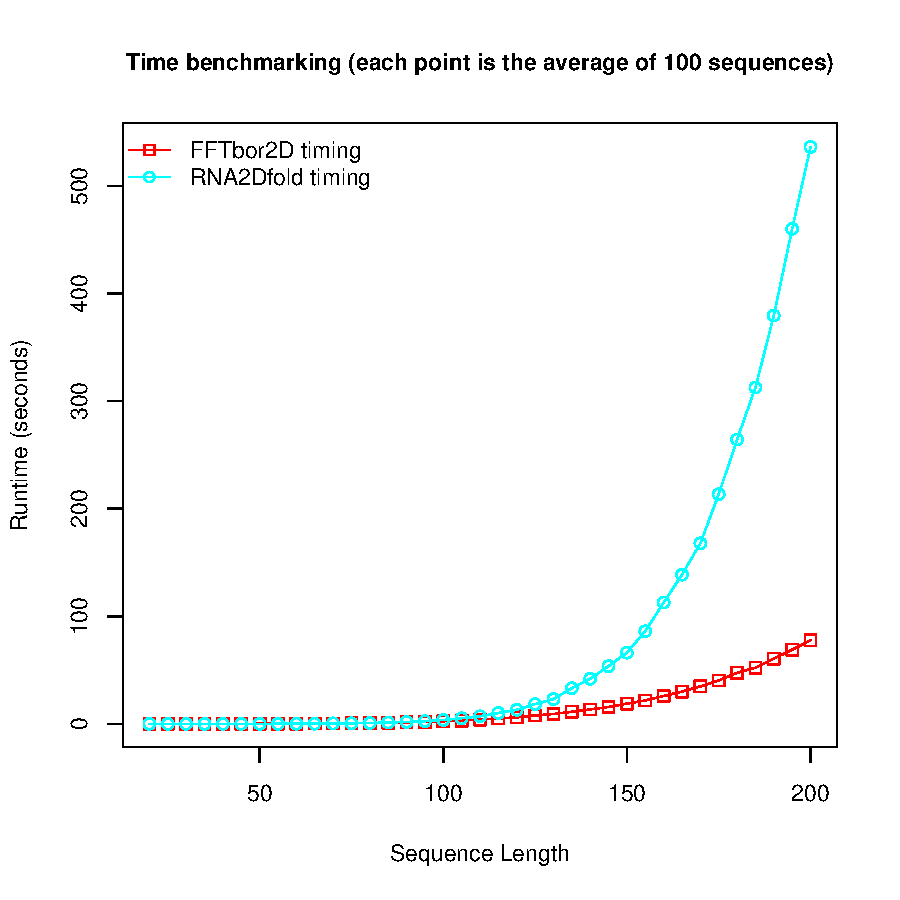
\includegraphics[width=.9\textwidth]{Figures/FFTbor2D/ffttwoRtwofoldTiming.pdf}
\caption[Run time in seconds for \rnatwofold and \ffttwo on random
RNA sequences of length 20--200 nt]{
Run time in seconds for \rnatwofold and \ffttwo on random
RNA sequences of length 20--200 nt, where sequence generation and
choice of metastable structures \strAB is described in the text.
Beyond a length of approximately 80 nt, \ffttwo is demonstrably
faster.
}
\label{fig:ffttwo:ffttwoRtwofoldTiming}
\end{figure}

\begin{figure}[!ht]
\centering
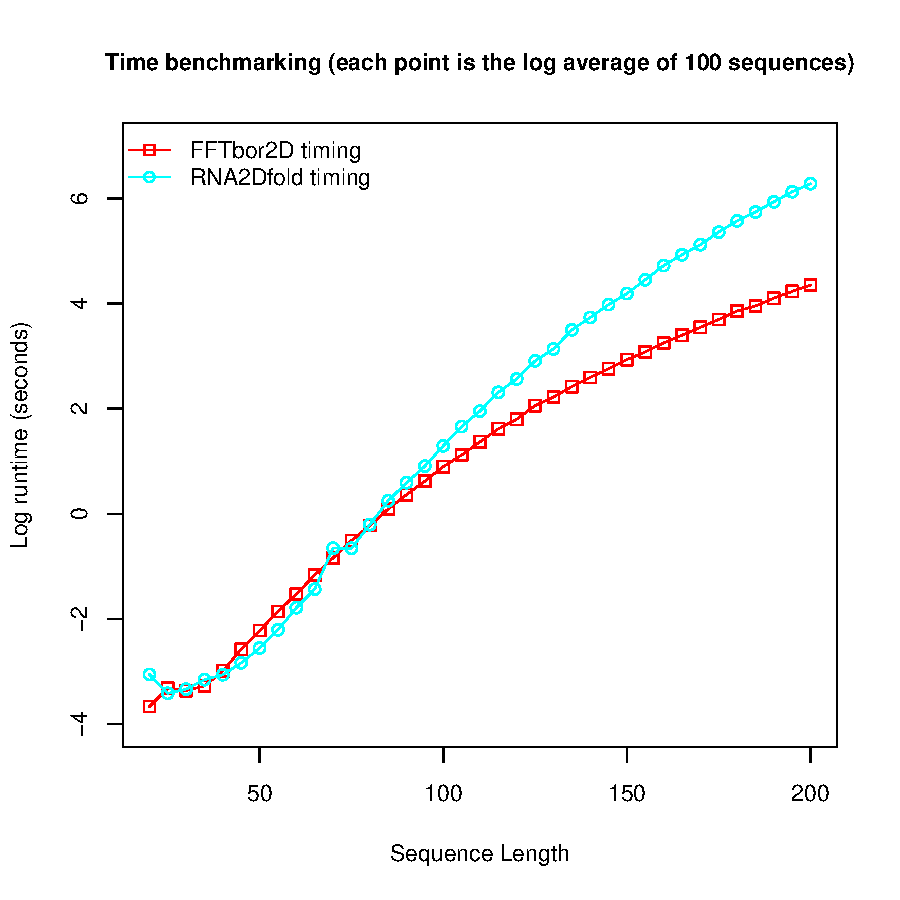
\includegraphics[width=.9\textwidth]{Figures/FFTbor2D/ffttwoRtwofoldLogScale.pdf}
\caption[Logarithm of run time in seconds for \rnatwofold and \ffttwo
on random RNA sequences of length less than 200 nt]{
Logarithm of run time in seconds for \rnatwofold and \ffttwo
on random RNA sequences of length less than 200 nt, for same data as that
in \Figref{ffttwo:ffttwoRtwofoldTiming}.
By taking $\log_{10}$ of the run times,
crossover points are apparent,
where \ffttwo is faster than \rnatwofold. For very small
sequences, \rnatwofold is faster, though since both programs converge
in a fraction of a second, this difference is of no practical consequence.
}
\label{fig:ffttwo:ffttwoRtwofoldLogScale}
\end{figure}

\begin{figure}[!ht]
\centering
\begin{subfigure}[h]{\textwidth}
\centering
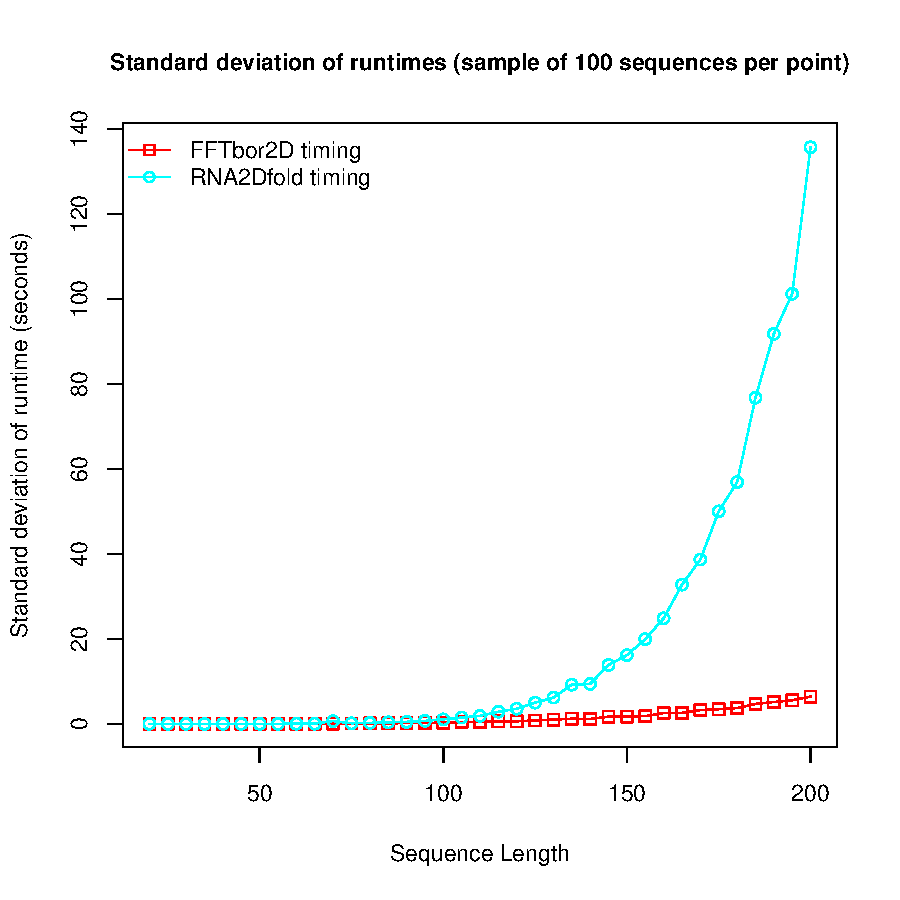
\includegraphics[width=.65\textwidth]{Figures/FFTbor2D/ffttwoRtwofoldStdev.pdf}
\end{subfigure} \\
\begin{subfigure}[h]{\textwidth}
\centering
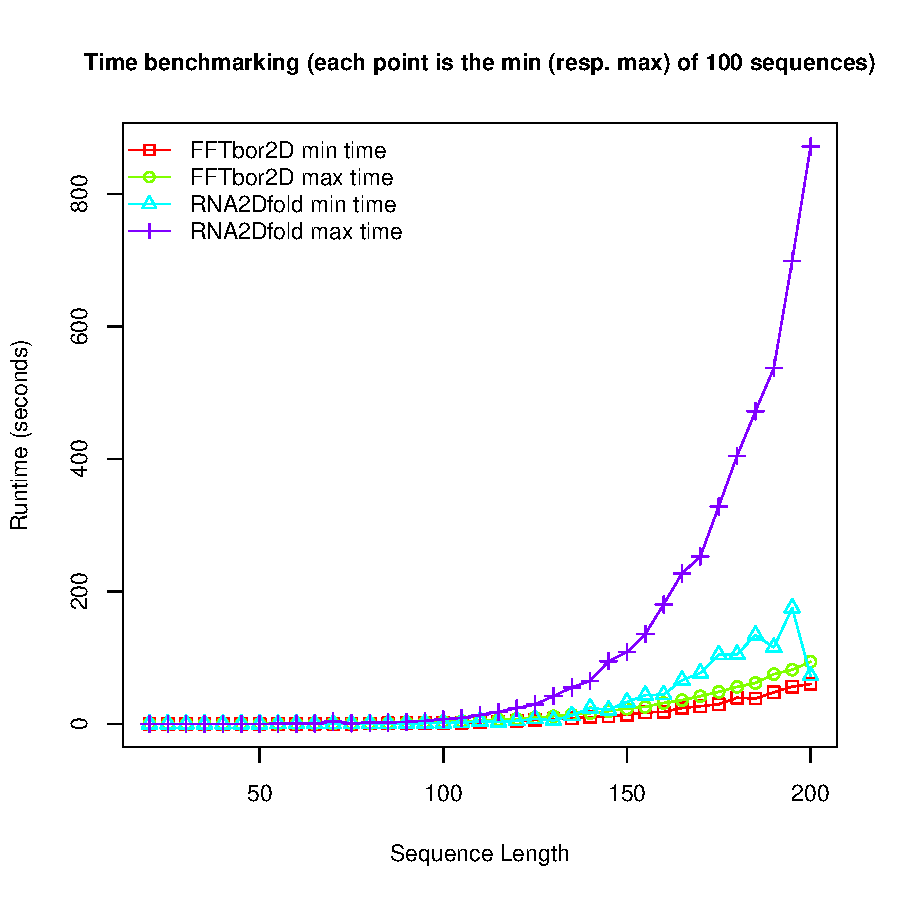
\includegraphics[width=.65\textwidth]{Figures/FFTbor2D/ffttwoRtwofoldMinMax.pdf}
\end{subfigure}
\caption[{\em (Top)}
Standard deviation of run times of \rnatwofold and \ffttwo
as a function of sequence length $n$.
{\em (Bottom)}
Minimum and maximum run times for \rnatwofold and \ffttwo]{
{\em (Top)}
Standard deviation of run times of \rnatwofold and \ffttwo
as a function of sequence length $n$.
{\em (Bottom)}
Minimum and maximum run times for \rnatwofold and \ffttwo.
For each collection of 100 random sequences of length $n$, the minimum
and maximum run time for a sequence of that length was computed.
Taken together, these figures clearly show the
run time dependence of \rnatwofold on particular sequences, while
the run time of \ffttwo depends only on sequence length, rather than
sequence details.
}
\label{fig:ffttwo:ffttwoRtwofoldStdevMinMax}
\end{figure}

\begin{figure}[!ht]
\centering
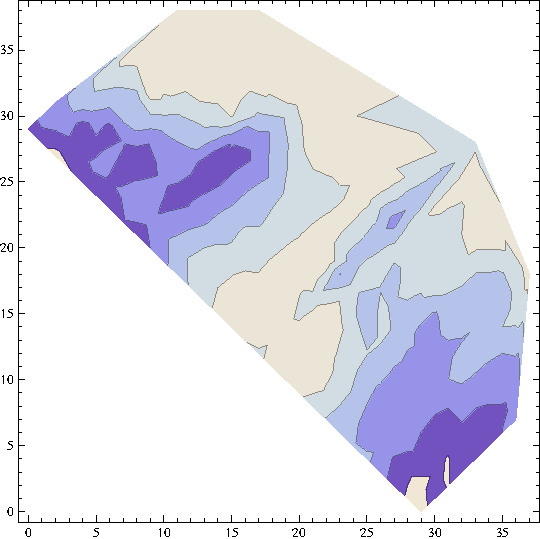
\includegraphics[width=.7\textwidth]{Figures/FFTbor2D/ffttwoProbContour.pdf}
\caption[2D projection of energy landscape for Spliced Leader (SL) RNA
from {\em L. collosoma}, as computed by \ffttwo]{
2D projection of energy landscape for Spliced Leader (SL) RNA
from {\em L. collosoma}, having
sequence and metastable secondary structures: \rule[-1.25em]{0pt}{0pt} \\
$\seq\,=$ \ms{AACUAAAACAAUUUUUGAAGAACAGUUUCUGUACUUCAUUGGUAUGUAGAGACUUC} \\
$\strA =$ \ms{..((...((((((..(((((.((((...)))).)))))..))).)))..)).....} \\
$\strB =$ \ms{.......................((((((((((((.....)))))..)))))))..}
\rule[-1.25em]{0pt}{0pt} \\
The $x$-axis [resp. $y$-axis]
represents \bpd between metastable structure \strA [resp.
\strBresp],
while the $z$-axis represents the ensemble free energy $-RT \log \bfZ{x,y}{}$,
where \bfZ{x,y}{} is computed in \ffttwo by $\bfZ{x,y}{}=p(x,y) \cdot \fullZ$.
Low energy positions $(x,y)$ correspond to high Boltzmann probability positions.
The left panel depicts a heat map of the ensemble free energy,
while the right panel depicts a contour map with level curves. In analogy
with mountain climbing, one expects an optimal path to follow along the
valley regions in traversing the landscape from \strA to \strB. Data produced
with \ffttwo; graphics produced using Mathematica.
}
\label{fig:ffttwo:ffttwoProbContour}
\end{figure}

\begin{figure}[!ht]
\centering
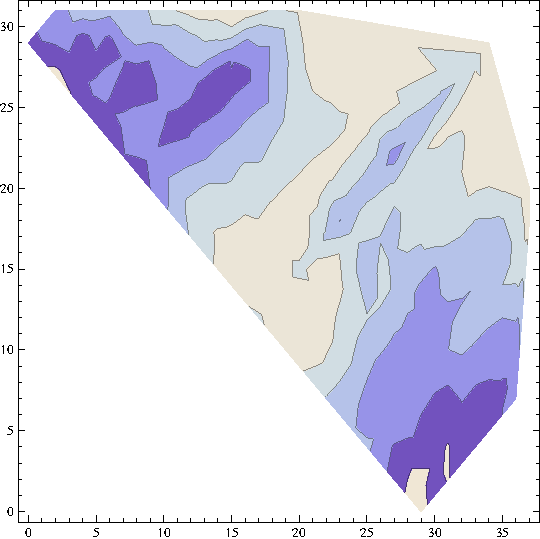
\includegraphics[width=.45\textwidth]{Figures/FFTbor2D/rtwofoldProbContour.pdf}
\quad
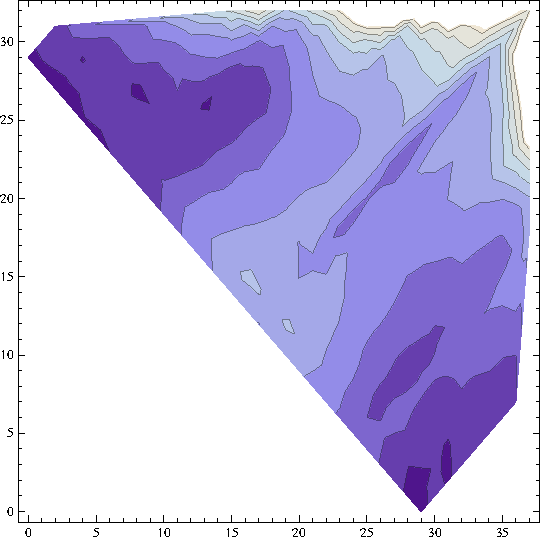
\includegraphics[width=.45\textwidth]{Figures/FFTbor2D/rtwofoldEnsFreeEnergyContour.pdf}
\caption[2D projection of energy landscape for Spliced Leader (SL) RNA
from {\em L. collosoma}, as in
\Figref{ffttwo:ffttwoProbContour},
except that in the right panel, ensemble free energy $-RT \log \bfZ{x,y}{}$
is computed from the values of \bfZ{x,y}{} output by \rnatwofold,
while in the left panel, ensemble free energy is computed from
the values $\bfZ{x,y}{}=p(x,y) \cdot \fullZ$, where values $p(x,y)$ are output
by \rnatwofold]{
2D projection of energy landscape for Spliced Leader (SL) RNA
from {\em L. collosoma}, as in
\Figref{ffttwo:ffttwoProbContour},
except that in the right panel, ensemble free energy $-RT \log \bfZ{x,y}{}$
is computed from the values of \bfZ{x,y}{} output by \rnatwofold,
while in the left panel, ensemble free energy is computed from
the values $\bfZ{x,y}{}=p(x,y) \cdot \fullZ$, where values $p(x,y)$ are output
by \rnatwofold.
The loss of detail in the 2D energy landscape is caused uniquely by
working with probabilities $p(x,y)$, rather than partition function
values \bfZ{x,y}{}.
Data produced with \rnatwofold; graphics produced using Mathematica.
}
\label{fig:ffttwo:rtwofoldProbContour}
\end{figure}

An important advantage of
\rnatwofold over \ffttwo is that the former can additionally
compute the structures $M_{x,y}$ having \mfe over all
structures that are $x$-neighbors of metastable \strA and simultaneously
$y$-neighbors of metastable \strB. (There is a similar advantage of \rnabor
\citep{freyhult.b07} over the faster \fftbor \citep{senter.po12}.)
As well, \rnatwofold directly computes the partition function values
\bfZ{x,y}{}, while \ffttwo estimates \bfZ{x,y}{} by computing
$p(x,y) \cdot \fullZ$. This difference entails a significant loss of precision,
when depicting the energy landscape.
